%% LyX 2.1.4 created this file.  For more info, see http://www.lyx.org/.
%% Do not edit unless you really know what you are doing.
\documentclass[english]{acmsmall}
\usepackage[latin9]{inputenc}
\setcounter{secnumdepth}{3}
\setcounter{tocdepth}{3}
\usepackage{graphicx}
\usepackage{babel}
\begin{document}

\title{Live orchestral piano}

\maketitle

\section{Live Orchestral Piano (LOP)}

We introduce in this section the \emph{Live Orchestral Piano} (LOP)
application, which is the first software able to provide a way to
compose music with a full classical orchestra in real-time by simply
playing on a MIDI piano. The goal of this framework is to rely on
the knowledge learned by the model introduced in the previous sections
in order to perform the projection from a piano melody to the orchestra.


\subsection{Workflow}

The software is implemented on a client/server paradigm. This choice
allows to separate the orchestral computation part from the interface
and sound rendering engine. That way, multiple interfaces can easily
be implemented. It should also be noted that separating the computing
and rendering on different computers, can allow to use high-quality
and CPU-intensive orchestral rendering plugins. This can allow a more
realistic orchestral rendering with heavy amounts of computation performed
while ensuring the real-time constraint on the overall system (preventing
degradation of the computing part). The complete implementation workflow
is presented in Figure~\ref{fig:Live-orchestral-piano}.

\begin{figure*}
\begin{centering}
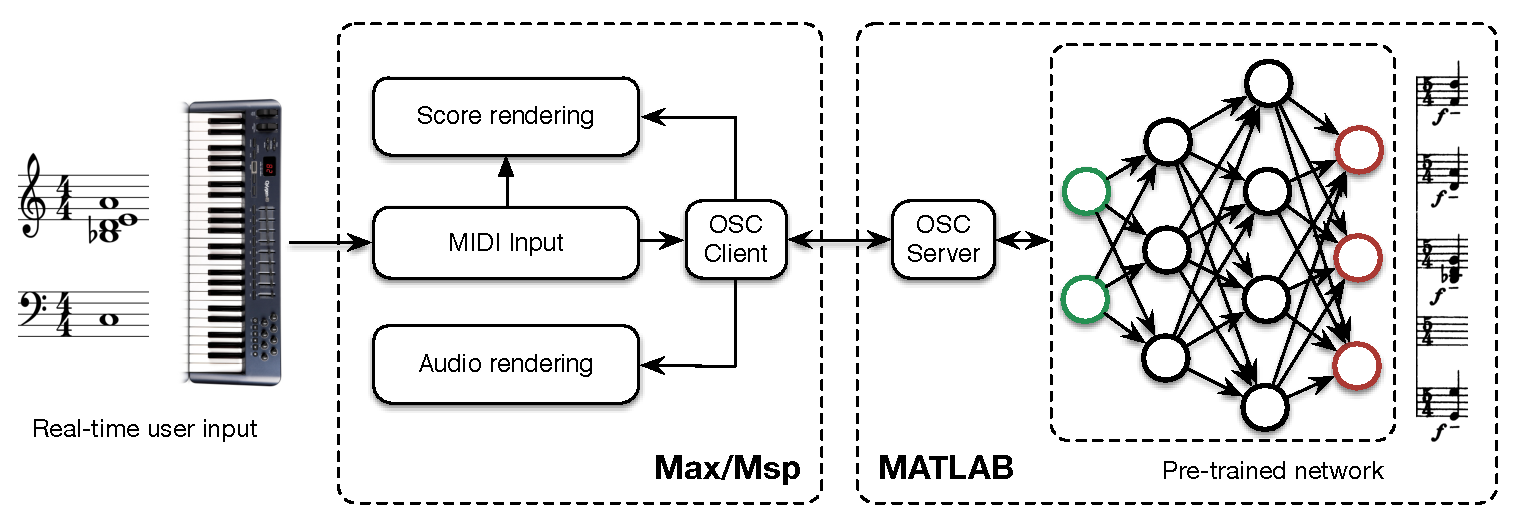
\includegraphics[scale=0.55]{workflow}
\par\end{centering}

\caption{\label{fig:Live-orchestral-piano}Live orchestral piano (L.O.P) implementation
workflow. The user inputs a melody which is transcribed into a score
and send via OSC from the Max/Msp client. Then, the MATLAB server
uses this vector of notes and process it following the aforementioned
techniques in order to obtain the orchestration. This information
is then sent back to Max/Msp which performs the real-time audio rendering }
\end{figure*}


As we can see, the user can input a melody (single notes or chords)
through a MIDI keyboard, which is retrieved inside the Max/Msp interface.
The interface transmits this symbolic information (as a variable-length
vector of active notes) via OSC to the MATLAB server. The interface
performs a real-time transcription of the piano score to the screen
in parallel. The server uses this vector of events to produce an 88
vector of binary input note activations (as defined in Section~\textbf{XXX}).
This vector is then processed by using the orchestration algorithms
presented in Section~\textbf{XXX} in order to obtain a projection
of a specific symbolic piano melody to the full orchestra (an operation
defined as \emph{projective orchestration}). The resulting orchestration
is then sent back to the client interface which performs both the
real-time audio rendering and score transcription. 

\textbf{NB: A good thing would be to compute the end-to-end latency
in the system ! And also to compute this with a variable number of
Gibbs steps ... all of this to show that we respect real-time constraints
/ requirements.}


\subsection{Interface}

The interface has been developed in Max/Msp, to facilitate both the
score and audio rendering aspects in a real-time environment. The
score rendering is handled by the \emph{Bach }library environment
\textbf{{[}INSERT REF{]}}. This interface provides a way to easily
switch between different orchestration models, while controling other
meta-parameters of the sampling. For instance the \emph{cutoff probability
}gives a direct access to the density of the generated orchestration
(in terms of number of played instruments). Indeed, a low cutoff probability
implies that most activation of notes will be taken into account in
the playback, while a high cutoff will produce more sparse orchestration.

\textbf{{[}INCLUDE FIGURE WITH LIVE EXAMPLE{]}}


\subsection{Examples\&}

Score and videos ?


\subsection{Offline generation}

Retry to generate full orchestral scores from piano scores. (with
new threshold and unit-variance transform) 

+ Assess various thresholds of generation

+ Try on Moussorgski and Beethoven
\end{document}
